\documentclass{article}
\usepackage[submission]{colm2026_conference}

\usepackage{microtype}
\usepackage{hyperref}
\usepackage{url}
\usepackage{booktabs}
\usepackage{graphicx}
\usepackage{amsmath}
\usepackage{amssymb}
\usepackage{tabularx}
\usepackage{makecell}
\usepackage{subcaption}
\usepackage{enumitem}
\usepackage{placeins}
\usepackage{xcolor}
\usepackage{lineno}

%%%%% NEW MATH DEFINITIONS %%%%%

\usepackage{amsmath,amsfonts,bm}

% Mark sections of captions for referring to divisions of figures
\newcommand{\figleft}{{\em (Left)}}
\newcommand{\figcenter}{{\em (Center)}}
\newcommand{\figright}{{\em (Right)}}
\newcommand{\figtop}{{\em (Top)}}
\newcommand{\figbottom}{{\em (Bottom)}}
\newcommand{\captiona}{{\em (a)}}
\newcommand{\captionb}{{\em (b)}}
\newcommand{\captionc}{{\em (c)}}
\newcommand{\captiond}{{\em (d)}}

% Highlight a newly defined term
\newcommand{\newterm}[1]{{\bf #1}}


% Figure reference, lower-case.
\def\figref#1{figure~\ref{#1}}
% Figure reference, capital. For start of sentence
\def\Figref#1{Figure~\ref{#1}}
\def\twofigref#1#2{figures \ref{#1} and \ref{#2}}
\def\quadfigref#1#2#3#4{figures \ref{#1}, \ref{#2}, \ref{#3} and \ref{#4}}
% Section reference, lower-case.
\def\secref#1{section~\ref{#1}}
% Section reference, capital.
\def\Secref#1{Section~\ref{#1}}
% Reference to two sections.
\def\twosecrefs#1#2{sections \ref{#1} and \ref{#2}}
% Reference to three sections.
\def\secrefs#1#2#3{sections \ref{#1}, \ref{#2} and \ref{#3}}
% Reference to an equation, lower-case.
\def\eqref#1{equation~\ref{#1}}
% Reference to an equation, upper case
\def\Eqref#1{Equation~\ref{#1}}
% A raw reference to an equation---avoid using if possible
\def\plaineqref#1{\ref{#1}}
% Reference to a chapter, lower-case.
\def\chapref#1{chapter~\ref{#1}}
% Reference to an equation, upper case.
\def\Chapref#1{Chapter~\ref{#1}}
% Reference to a range of chapters
\def\rangechapref#1#2{chapters\ref{#1}--\ref{#2}}
% Reference to an algorithm, lower-case.
\def\algref#1{algorithm~\ref{#1}}
% Reference to an algorithm, upper case.
\def\Algref#1{Algorithm~\ref{#1}}
\def\twoalgref#1#2{algorithms \ref{#1} and \ref{#2}}
\def\Twoalgref#1#2{Algorithms \ref{#1} and \ref{#2}}
% Reference to a part, lower case
\def\partref#1{part~\ref{#1}}
% Reference to a part, upper case
\def\Partref#1{Part~\ref{#1}}
\def\twopartref#1#2{parts \ref{#1} and \ref{#2}}

\def\ceil#1{\lceil #1 \rceil}
\def\floor#1{\lfloor #1 \rfloor}
\def\1{\bm{1}}
\newcommand{\train}{\mathcal{D}}
\newcommand{\valid}{\mathcal{D_{\mathrm{valid}}}}
\newcommand{\test}{\mathcal{D_{\mathrm{test}}}}

\def\eps{{\epsilon}}


% Random variables
\def\reta{{\textnormal{$\eta$}}}
\def\ra{{\textnormal{a}}}
\def\rb{{\textnormal{b}}}
\def\rc{{\textnormal{c}}}
\def\rd{{\textnormal{d}}}
\def\re{{\textnormal{e}}}
\def\rf{{\textnormal{f}}}
\def\rg{{\textnormal{g}}}
\def\rh{{\textnormal{h}}}
\def\ri{{\textnormal{i}}}
\def\rj{{\textnormal{j}}}
\def\rk{{\textnormal{k}}}
\def\rl{{\textnormal{l}}}
% rm is already a command, just don't name any random variables m
\def\rn{{\textnormal{n}}}
\def\ro{{\textnormal{o}}}
\def\rp{{\textnormal{p}}}
\def\rq{{\textnormal{q}}}
\def\rr{{\textnormal{r}}}
\def\rs{{\textnormal{s}}}
\def\rt{{\textnormal{t}}}
\def\ru{{\textnormal{u}}}
\def\rv{{\textnormal{v}}}
\def\rw{{\textnormal{w}}}
\def\rx{{\textnormal{x}}}
\def\ry{{\textnormal{y}}}
\def\rz{{\textnormal{z}}}

% Random vectors
\def\rvepsilon{{\mathbf{\epsilon}}}
\def\rvtheta{{\mathbf{\theta}}}
\def\rva{{\mathbf{a}}}
\def\rvb{{\mathbf{b}}}
\def\rvc{{\mathbf{c}}}
\def\rvd{{\mathbf{d}}}
\def\rve{{\mathbf{e}}}
\def\rvf{{\mathbf{f}}}
\def\rvg{{\mathbf{g}}}
\def\rvh{{\mathbf{h}}}
\def\rvu{{\mathbf{i}}}
\def\rvj{{\mathbf{j}}}
\def\rvk{{\mathbf{k}}}
\def\rvl{{\mathbf{l}}}
\def\rvm{{\mathbf{m}}}
\def\rvn{{\mathbf{n}}}
\def\rvo{{\mathbf{o}}}
\def\rvp{{\mathbf{p}}}
\def\rvq{{\mathbf{q}}}
\def\rvr{{\mathbf{r}}}
\def\rvs{{\mathbf{s}}}
\def\rvt{{\mathbf{t}}}
\def\rvu{{\mathbf{u}}}
\def\rvv{{\mathbf{v}}}
\def\rvw{{\mathbf{w}}}
\def\rvx{{\mathbf{x}}}
\def\rvy{{\mathbf{y}}}
\def\rvz{{\mathbf{z}}}

% Elements of random vectors
\def\erva{{\textnormal{a}}}
\def\ervb{{\textnormal{b}}}
\def\ervc{{\textnormal{c}}}
\def\ervd{{\textnormal{d}}}
\def\erve{{\textnormal{e}}}
\def\ervf{{\textnormal{f}}}
\def\ervg{{\textnormal{g}}}
\def\ervh{{\textnormal{h}}}
\def\ervi{{\textnormal{i}}}
\def\ervj{{\textnormal{j}}}
\def\ervk{{\textnormal{k}}}
\def\ervl{{\textnormal{l}}}
\def\ervm{{\textnormal{m}}}
\def\ervn{{\textnormal{n}}}
\def\ervo{{\textnormal{o}}}
\def\ervp{{\textnormal{p}}}
\def\ervq{{\textnormal{q}}}
\def\ervr{{\textnormal{r}}}
\def\ervs{{\textnormal{s}}}
\def\ervt{{\textnormal{t}}}
\def\ervu{{\textnormal{u}}}
\def\ervv{{\textnormal{v}}}
\def\ervw{{\textnormal{w}}}
\def\ervx{{\textnormal{x}}}
\def\ervy{{\textnormal{y}}}
\def\ervz{{\textnormal{z}}}

% Random matrices
\def\rmA{{\mathbf{A}}}
\def\rmB{{\mathbf{B}}}
\def\rmC{{\mathbf{C}}}
\def\rmD{{\mathbf{D}}}
\def\rmE{{\mathbf{E}}}
\def\rmF{{\mathbf{F}}}
\def\rmG{{\mathbf{G}}}
\def\rmH{{\mathbf{H}}}
\def\rmI{{\mathbf{I}}}
\def\rmJ{{\mathbf{J}}}
\def\rmK{{\mathbf{K}}}
\def\rmL{{\mathbf{L}}}
\def\rmM{{\mathbf{M}}}
\def\rmN{{\mathbf{N}}}
\def\rmO{{\mathbf{O}}}
\def\rmP{{\mathbf{P}}}
\def\rmQ{{\mathbf{Q}}}
\def\rmR{{\mathbf{R}}}
\def\rmS{{\mathbf{S}}}
\def\rmT{{\mathbf{T}}}
\def\rmU{{\mathbf{U}}}
\def\rmV{{\mathbf{V}}}
\def\rmW{{\mathbf{W}}}
\def\rmX{{\mathbf{X}}}
\def\rmY{{\mathbf{Y}}}
\def\rmZ{{\mathbf{Z}}}

% Elements of random matrices
\def\ermA{{\textnormal{A}}}
\def\ermB{{\textnormal{B}}}
\def\ermC{{\textnormal{C}}}
\def\ermD{{\textnormal{D}}}
\def\ermE{{\textnormal{E}}}
\def\ermF{{\textnormal{F}}}
\def\ermG{{\textnormal{G}}}
\def\ermH{{\textnormal{H}}}
\def\ermI{{\textnormal{I}}}
\def\ermJ{{\textnormal{J}}}
\def\ermK{{\textnormal{K}}}
\def\ermL{{\textnormal{L}}}
\def\ermM{{\textnormal{M}}}
\def\ermN{{\textnormal{N}}}
\def\ermO{{\textnormal{O}}}
\def\ermP{{\textnormal{P}}}
\def\ermQ{{\textnormal{Q}}}
\def\ermR{{\textnormal{R}}}
\def\ermS{{\textnormal{S}}}
\def\ermT{{\textnormal{T}}}
\def\ermU{{\textnormal{U}}}
\def\ermV{{\textnormal{V}}}
\def\ermW{{\textnormal{W}}}
\def\ermX{{\textnormal{X}}}
\def\ermY{{\textnormal{Y}}}
\def\ermZ{{\textnormal{Z}}}

% Vectors
\def\vzero{{\bm{0}}}
\def\vone{{\bm{1}}}
\def\vmu{{\bm{\mu}}}
\def\vtheta{{\bm{\theta}}}
\def\va{{\bm{a}}}
\def\vb{{\bm{b}}}
\def\vc{{\bm{c}}}
\def\vd{{\bm{d}}}
\def\ve{{\bm{e}}}
\def\vf{{\bm{f}}}
\def\vg{{\bm{g}}}
\def\vh{{\bm{h}}}
\def\vi{{\bm{i}}}
\def\vj{{\bm{j}}}
\def\vk{{\bm{k}}}
\def\vl{{\bm{l}}}
\def\vm{{\bm{m}}}
\def\vn{{\bm{n}}}
\def\vo{{\bm{o}}}
\def\vp{{\bm{p}}}
\def\vq{{\bm{q}}}
\def\vr{{\bm{r}}}
\def\vs{{\bm{s}}}
\def\vt{{\bm{t}}}
\def\vu{{\bm{u}}}
\def\vv{{\bm{v}}}
\def\vw{{\bm{w}}}
\def\vx{{\bm{x}}}
\def\vy{{\bm{y}}}
\def\vz{{\bm{z}}}

% Elements of vectors
\def\evalpha{{\alpha}}
\def\evbeta{{\beta}}
\def\evepsilon{{\epsilon}}
\def\evlambda{{\lambda}}
\def\evomega{{\omega}}
\def\evmu{{\mu}}
\def\evpsi{{\psi}}
\def\evsigma{{\sigma}}
\def\evtheta{{\theta}}
\def\eva{{a}}
\def\evb{{b}}
\def\evc{{c}}
\def\evd{{d}}
\def\eve{{e}}
\def\evf{{f}}
\def\evg{{g}}
\def\evh{{h}}
\def\evi{{i}}
\def\evj{{j}}
\def\evk{{k}}
\def\evl{{l}}
\def\evm{{m}}
\def\evn{{n}}
\def\evo{{o}}
\def\evp{{p}}
\def\evq{{q}}
\def\evr{{r}}
\def\evs{{s}}
\def\evt{{t}}
\def\evu{{u}}
\def\evv{{v}}
\def\evw{{w}}
\def\evx{{x}}
\def\evy{{y}}
\def\evz{{z}}

% Matrix
\def\mA{{\bm{A}}}
\def\mB{{\bm{B}}}
\def\mC{{\bm{C}}}
\def\mD{{\bm{D}}}
\def\mE{{\bm{E}}}
\def\mF{{\bm{F}}}
\def\mG{{\bm{G}}}
\def\mH{{\bm{H}}}
\def\mI{{\bm{I}}}
\def\mJ{{\bm{J}}}
\def\mK{{\bm{K}}}
\def\mL{{\bm{L}}}
\def\mM{{\bm{M}}}
\def\mN{{\bm{N}}}
\def\mO{{\bm{O}}}
\def\mP{{\bm{P}}}
\def\mQ{{\bm{Q}}}
\def\mR{{\bm{R}}}
\def\mS{{\bm{S}}}
\def\mT{{\bm{T}}}
\def\mU{{\bm{U}}}
\def\mV{{\bm{V}}}
\def\mW{{\bm{W}}}
\def\mX{{\bm{X}}}
\def\mY{{\bm{Y}}}
\def\mZ{{\bm{Z}}}
\def\mBeta{{\bm{\beta}}}
\def\mPhi{{\bm{\Phi}}}
\def\mLambda{{\bm{\Lambda}}}
\def\mSigma{{\bm{\Sigma}}}

% Tensor
\DeclareMathAlphabet{\mathsfit}{\encodingdefault}{\sfdefault}{m}{sl}
\SetMathAlphabet{\mathsfit}{bold}{\encodingdefault}{\sfdefault}{bx}{n}
\newcommand{\tens}[1]{\bm{\mathsfit{#1}}}
\def\tA{{\tens{A}}}
\def\tB{{\tens{B}}}
\def\tC{{\tens{C}}}
\def\tD{{\tens{D}}}
\def\tE{{\tens{E}}}
\def\tF{{\tens{F}}}
\def\tG{{\tens{G}}}
\def\tH{{\tens{H}}}
\def\tI{{\tens{I}}}
\def\tJ{{\tens{J}}}
\def\tK{{\tens{K}}}
\def\tL{{\tens{L}}}
\def\tM{{\tens{M}}}
\def\tN{{\tens{N}}}
\def\tO{{\tens{O}}}
\def\tP{{\tens{P}}}
\def\tQ{{\tens{Q}}}
\def\tR{{\tens{R}}}
\def\tS{{\tens{S}}}
\def\tT{{\tens{T}}}
\def\tU{{\tens{U}}}
\def\tV{{\tens{V}}}
\def\tW{{\tens{W}}}
\def\tX{{\tens{X}}}
\def\tY{{\tens{Y}}}
\def\tZ{{\tens{Z}}}


% Graph
\def\gA{{\mathcal{A}}}
\def\gB{{\mathcal{B}}}
\def\gC{{\mathcal{C}}}
\def\gD{{\mathcal{D}}}
\def\gE{{\mathcal{E}}}
\def\gF{{\mathcal{F}}}
\def\gG{{\mathcal{G}}}
\def\gH{{\mathcal{H}}}
\def\gI{{\mathcal{I}}}
\def\gJ{{\mathcal{J}}}
\def\gK{{\mathcal{K}}}
\def\gL{{\mathcal{L}}}
\def\gM{{\mathcal{M}}}
\def\gN{{\mathcal{N}}}
\def\gO{{\mathcal{O}}}
\def\gP{{\mathcal{P}}}
\def\gQ{{\mathcal{Q}}}
\def\gR{{\mathcal{R}}}
\def\gS{{\mathcal{S}}}
\def\gT{{\mathcal{T}}}
\def\gU{{\mathcal{U}}}
\def\gV{{\mathcal{V}}}
\def\gW{{\mathcal{W}}}
\def\gX{{\mathcal{X}}}
\def\gY{{\mathcal{Y}}}
\def\gZ{{\mathcal{Z}}}

% Sets
\def\sA{{\mathbb{A}}}
\def\sB{{\mathbb{B}}}
\def\sC{{\mathbb{C}}}
\def\sD{{\mathbb{D}}}
% Don't use a set called E, because this would be the same as our symbol
% for expectation.
\def\sF{{\mathbb{F}}}
\def\sG{{\mathbb{G}}}
\def\sH{{\mathbb{H}}}
\def\sI{{\mathbb{I}}}
\def\sJ{{\mathbb{J}}}
\def\sK{{\mathbb{K}}}
\def\sL{{\mathbb{L}}}
\def\sM{{\mathbb{M}}}
\def\sN{{\mathbb{N}}}
\def\sO{{\mathbb{O}}}
\def\sP{{\mathbb{P}}}
\def\sQ{{\mathbb{Q}}}
\def\sR{{\mathbb{R}}}
\def\sS{{\mathbb{S}}}
\def\sT{{\mathbb{T}}}
\def\sU{{\mathbb{U}}}
\def\sV{{\mathbb{V}}}
\def\sW{{\mathbb{W}}}
\def\sX{{\mathbb{X}}}
\def\sY{{\mathbb{Y}}}
\def\sZ{{\mathbb{Z}}}

% Entries of a matrix
\def\emLambda{{\Lambda}}
\def\emA{{A}}
\def\emB{{B}}
\def\emC{{C}}
\def\emD{{D}}
\def\emE{{E}}
\def\emF{{F}}
\def\emG{{G}}
\def\emH{{H}}
\def\emI{{I}}
\def\emJ{{J}}
\def\emK{{K}}
\def\emL{{L}}
\def\emM{{M}}
\def\emN{{N}}
\def\emO{{O}}
\def\emP{{P}}
\def\emQ{{Q}}
\def\emR{{R}}
\def\emS{{S}}
\def\emT{{T}}
\def\emU{{U}}
\def\emV{{V}}
\def\emW{{W}}
\def\emX{{X}}
\def\emY{{Y}}
\def\emZ{{Z}}
\def\emSigma{{\Sigma}}

% entries of a tensor
% Same font as tensor, without \bm wrapper
\newcommand{\etens}[1]{\mathsfit{#1}}
\def\etLambda{{\etens{\Lambda}}}
\def\etA{{\etens{A}}}
\def\etB{{\etens{B}}}
\def\etC{{\etens{C}}}
\def\etD{{\etens{D}}}
\def\etE{{\etens{E}}}
\def\etF{{\etens{F}}}
\def\etG{{\etens{G}}}
\def\etH{{\etens{H}}}
\def\etI{{\etens{I}}}
\def\etJ{{\etens{J}}}
\def\etK{{\etens{K}}}
\def\etL{{\etens{L}}}
\def\etM{{\etens{M}}}
\def\etN{{\etens{N}}}
\def\etO{{\etens{O}}}
\def\etP{{\etens{P}}}
\def\etQ{{\etens{Q}}}
\def\etR{{\etens{R}}}
\def\etS{{\etens{S}}}
\def\etT{{\etens{T}}}
\def\etU{{\etens{U}}}
\def\etV{{\etens{V}}}
\def\etW{{\etens{W}}}
\def\etX{{\etens{X}}}
\def\etY{{\etens{Y}}}
\def\etZ{{\etens{Z}}}

% The true underlying data generating distribution
\newcommand{\pdata}{p_{\rm{data}}}
% The empirical distribution defined by the training set
\newcommand{\ptrain}{\hat{p}_{\rm{data}}}
\newcommand{\Ptrain}{\hat{P}_{\rm{data}}}
% The model distribution
\newcommand{\pmodel}{p_{\rm{model}}}
\newcommand{\Pmodel}{P_{\rm{model}}}
\newcommand{\ptildemodel}{\tilde{p}_{\rm{model}}}
% Stochastic autoencoder distributions
\newcommand{\pencode}{p_{\rm{encoder}}}
\newcommand{\pdecode}{p_{\rm{decoder}}}
\newcommand{\precons}{p_{\rm{reconstruct}}}

\newcommand{\laplace}{\mathrm{Laplace}} % Laplace distribution

\newcommand{\E}{\mathbb{E}}
\newcommand{\Ls}{\mathcal{L}}
\newcommand{\R}{\mathbb{R}}
\newcommand{\emp}{\tilde{p}}
\newcommand{\lr}{\alpha}
\newcommand{\reg}{\lambda}
\newcommand{\rect}{\mathrm{rectifier}}
\newcommand{\softmax}{\mathrm{softmax}}
\newcommand{\sigmoid}{\sigma}
\newcommand{\softplus}{\zeta}
\newcommand{\KL}{D_{\mathrm{KL}}}
\newcommand{\Var}{\mathrm{Var}}
\newcommand{\standarderror}{\mathrm{SE}}
\newcommand{\Cov}{\mathrm{Cov}}
% Wolfram Mathworld says $L^2$ is for function spaces and $\ell^2$ is for vectors
% But then they seem to use $L^2$ for vectors throughout the site, and so does
% wikipedia.
\newcommand{\normlzero}{L^0}
\newcommand{\normlone}{L^1}
\newcommand{\normltwo}{L^2}
\newcommand{\normlp}{L^p}
\newcommand{\normmax}{L^\infty}

\newcommand{\parents}{Pa} % See usage in notation.tex. Chosen to match Daphne's book.

\DeclareMathOperator*{\argmax}{arg\,max}
\DeclareMathOperator*{\argmin}{arg\,min}

\DeclareMathOperator{\sign}{sign}
\DeclareMathOperator{\Tr}{Tr}
\let\ab\allowbreak

% Auto-generated by scripts/paper/build_colm2026_assets.py
\newcommand{\MergedRunId}{paper\_merged\_9x1000\_20260330T122258Z}
\newcommand{\PreparedExampleCount}{989}
\newcommand{\ScoreRowCount}{53,406}
\newcommand{\MetricRowCount}{53,406}
\newcommand{\SemanticIdentityValidCases}{7,242}
\newcommand{\PooledLagMedian}{21.0}
\newcommand{\PooledLagCILow}{20.0}
\newcommand{\PooledLagCIHigh}{21.0}
\newcommand{\FlagshipTwentyPlausiblePct}{72\%}
\newcommand{\FlagshipTwentyCommittedPct}{4\%}
\newcommand{\FlagshipFiftyPlausiblePct}{86\%}
\newcommand{\FlagshipFiftyCommittedPct}{9\%}
\newcommand{\FlagshipEightyPlausiblePct}{94\%}
\newcommand{\FlagshipEightyCommittedPct}{30\%}
\newcommand{\PaperPromptCount}{989}
\newcommand{\ArcPromptCount}{195}
\newcommand{\CsqaPromptCount}{794}
\newcommand{\OverallPrimaryPositiveCells}{18}
\newcommand{\OverallPrimaryEvaluableCells}{18}
\newcommand{\OverallPrimaryInsufficientCells}{0}
\newcommand{\OverallSecondaryPositiveCells}{18}
\newcommand{\OverallSecondaryEvaluableCells}{18}
\newcommand{\OverallSecondaryInsufficientCells}{0}
\newcommand{\ArcCsqaPositiveCells}{18}
\newcommand{\ArcCsqaEvaluableCells}{18}
\newcommand{\GoldArcCsqaPositiveCells}{18}
\newcommand{\GoldArcCsqaEvaluableCells}{18}
\newcommand{\SemanticIdentityValidRate}{81\%}
\newcommand{\TemplatedIdentityValidRate}{58\%}
\newcommand{\LetterIdentityValidRate}{95\%}
\newcommand{\TemplatedAgreementIdentity}{60\%}
\newcommand{\LetterAgreementIdentity}{44\%}
\newcommand{\AllSameReadoutRate}{31\%}
\newcommand{\SemanticPairedLagMedian}{nan}
\newcommand{\TemplatedPairedLagMedian}{nan}
\newcommand{\LetterPairedLagMedian}{nan}
\newcommand{\SemanticPairedPositivePct}{78\%}
\newcommand{\TemplatedPairedPositivePct}{58\%}
\newcommand{\LetterPairedPositivePct}{95\%}
\newcommand{\DuplicateOptionCount}{17}
\newcommand{\TokenCollisionCount}{1224}


\graphicspath{{figures/}}

\definecolor{darkblue}{rgb}{0, 0, 0.5}
\hypersetup{colorlinks=true, citecolor=darkblue, linkcolor=darkblue, urlcolor=darkblue}

\title{When Models Commit: Candidate Formation and Winner Isolation Across Model Depth}
\author{Anonymous Authors}

\begin{document}

\ifcolmsubmission
\linenumbers
\fi

\maketitle

\begin{abstract}
Language models produce one answer, but they need not arrive there in one step: an answer can become plausible before it becomes decisive. We study that gap in multiple-choice question answering by scoring exact option-text continuations layer by layer in nine instruction-tuned open-weight models from the Qwen, Gemma, and Llama families on \PaperPromptCount{} ARC-Challenge and CommonsenseQA questions. For each prompt, we measure when the eventual answer first enters a small plausible-answer set and when it later opens a stable margin over the runner-up. The gap is large and consistent. By 20\% of normalized depth, the eventual answer is already plausible in \FlagshipTwentyPlausiblePct{} of evaluable cases, but it is already committed in only \FlagshipTwentyCommittedPct{}; every evaluable model-dataset cell is positive under the preregistered primary rule. Two control readouts show the same broad pattern while changing which cases are measurable and, often, which answer wins. In the setting we study, candidate formation usually comes earlier than winner isolation.
\end{abstract}

\section{Introduction}

A multiple-choice answer hides more than one decision. A model can first narrow the field to a few answers that still seem possible and only later settle on one final winner. Standard evaluation only shows the last step. It tells us what answer came out, but not when that answer first became a serious option inside the network.

This paper asks a simple question. Does the eventual answer become one of the plausible answers before the model writes the margin that finally separates it from the runner-up? Figure~\ref{fig:flagship} previews the answer. In the pooled primary analysis, by 20\% of normalized depth the eventual answer is already in the plausible answer set for \FlagshipTwentyPlausiblePct{} of evaluable cases, but only \FlagshipTwentyCommittedPct{} are already stably committed.

We answer that question in a deliberately direct way. We build a normal multiple-choice
prompt, end it with the suffix ``\texttt{Final answer:}'', and then score the exact strings the
model could write next. On the main path, that string is the full option text itself, such
as ``\texttt{photosynthesis}''. So instead of training a separate probe to guess the answer
from hidden states, we measure the scores of the answer strings that the model is actually
being asked to produce.

Our setting is intentionally narrow and easy to audit. We evaluate nine instruction-tuned
open-weight models from the Qwen 2.5 Instruct, Gemma 2 IT, and Llama Instruct families
on \PaperPromptCount{} ARC-Challenge and CommonsenseQA questions. The claim of the
paper is limited to that setting. Within it, the pattern is consistent: the eventual answer
usually enters the plausible answer set well before it becomes stably isolated from the
runner-up. All \ArcCsqaPositiveCells{} evaluable model-dataset cells are positive under the
preregistered primary rule (Figure~\ref{fig:forest}, Table~\ref{tab:primary-summary}).

The paper makes three contributions. First, it gives a simple measurement framework for
separating ``still possible'' from ``finally chosen'' by scoring the task's own answer strings
rather than an external probe target. Second, it shows a large and consistent gap between
those two stages in the pooled curves and in every evaluable ARC-Challenge and
CommonsenseQA cell. Third, it shows that the same broad lag remains visible under two
control answer formats, even though those controls change coverage and can change the
final winner.

\begin{figure*}[t]
\centering
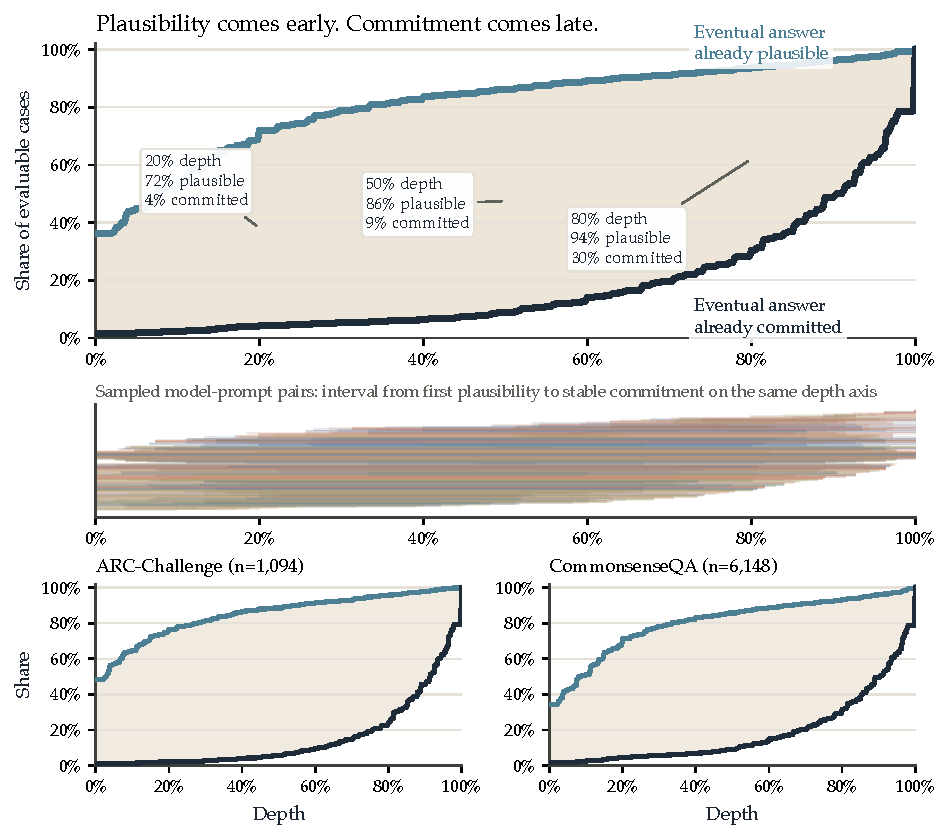
\includegraphics[width=\textwidth]{figure1_flagship_plausibility_commitment.pdf}
\caption{\textbf{The eventual answer becomes plausible much earlier than it becomes committed.} The top panel pools all evaluable model-prompt pairs from the primary analysis path (\texttt{semantic\_exact} with identity ordering). The light curve asks: by this depth, in how many cases is the eventual answer already one of the plausible answers? The dark curve asks: by this depth, in how many cases has the model already opened a stable winner-runner margin that it keeps through the end of the network? The band between the curves is the main object in the paper: cases where the answer already looks plausible but the model has not fully committed yet. The interval strip shows a sample of individual cases on the same normalized-depth axis, and the two bottom panels show the same pattern separately for ARC-Challenge and CommonsenseQA.}
\label{fig:flagship}
\end{figure*}

\section{Setup and measurement}

Table~\ref{tab:design-summary} summarizes the experiment design. The model panel contains
nine instruction-tuned checkpoints from three families: Qwen 2.5 Instruct~\citep{qwen25card},
Gemma 2 IT~\citep{gemma2card}, and Llama Instruct~\citep{llama3herd}. The reported
benchmark slice contains \ArcPromptCount{} ARC-Challenge prompts~\citep{clark2018arc}
and \CsqaPromptCount{} CommonsenseQA prompts~\citep{talmor2019commonsenseqa}.

For every model, we render a normal multiple-choice prompt and end it with the literal
suffix ``\texttt{Final answer:}''. After that suffix, we score three possible continuations:
\begin{itemize}[leftmargin=1.2em, itemsep=0.2em, topsep=0.35em]
\item the exact option text itself, such as ``\texttt{photosynthesis}'';
\item the literal template ``\texttt{The answer is \{option\_text\}}'';
\item the bare answer letter, such as ``\texttt{A}''.
\end{itemize}
The exact option-text path is the preregistered primary analysis. The other two are controls.
They keep the same prompt and the same answer choices, but they change which exact
continuation string we score after ``\texttt{Final answer:}''.

\begin{table*}[t]
\centering
\small
\begin{tabularx}{\linewidth}{@{}lX@{}}
\toprule
\textbf{Aspect} & \textbf{Configuration}\\
\midrule
Models & Nine instruction-tuned checkpoints from Qwen 2.5 Instruct (1.5B, 3B, 7B), Gemma 2 IT (2B, 9B, 27B), and Llama Instruct (3.2 1B, 3.2 3B, 3.1 8B). \\
Dataset slice & ARC-Challenge (195) and CommonsenseQA (794). \\
Prompting & Model-specific chat or raw prompt templates. Every prompt ends with the literal suffix ``\texttt{Final answer:}''. \\
Readouts & Primary: the exact option text after ``\texttt{Final answer:}'', for example ``\texttt{photosynthesis}''. Controls: the literal continuation ``\texttt{The answer is \{option\_text\}}'' and the bare answer letter, such as ``\texttt{A}''. \\
Permutations & Identity ordering and reverse ordering, kept paired on the same example subset. \\
Primary rule & For each model-dataset cell, report the median commitment lag $\Delta_{\mathrm{margin}} = d_{\mathrm{margin}} - d_{\mathrm{id}}$ with a grouped-bootstrap 95\% confidence interval; the cell is positive iff the lower confidence bound is greater than zero. \\
\bottomrule
\end{tabularx}

\caption{\textbf{Reader-facing summary of the experiment design.} The main question stays fixed throughout the paper: scoring the exact option text is primary, the two alternative continuation strings are controls, and identity versus reverse answer order is kept paired on the same example subset.}
\label{tab:design-summary}
\end{table*}

We score these continuations under teacher forcing, one layer at a time. In practical terms,
we do not let the model free-generate a long answer. We stop at ``\texttt{Final answer:}''
and ask how much probability the network assigns to each allowed continuation at each
layer. Let $p_\ell(o)$ denote the normalized probability of option $o$ at layer $\ell$. We
sort options by $p_\ell(o)$ and define a plausible answer set $C_\ell$ as the smallest prefix
whose cumulative probability reaches $\tau = 0.8$. If the cutoff lands inside a numerical tie,
we mark that layer as ambiguous instead of forcing an arbitrary choice. In words, $C_\ell$
is the small set of answers that the model still treats as seriously possible at layer $\ell$.

Our primary anchor is the \emph{eventual answer}, meaning the option that wins at the final layer under the primary readout. Denote it by $o^\star$. We then track three depth events:
\begin{align}
d_{\mathrm{id}} &= \min \{\ell : o^\star \in C_\ell\}, \\
d_{\mathrm{top1}} &= \min \{\ell : o^\star \text{ is the unique top-1 option at every later layer}\}, \\
d_{\mathrm{margin}} &= \min \{\ell : p_t(o^\star) - p_t(o_{(2)}) \ge \delta \text{ for all } t \ge \ell\},
\end{align}
where $o_{(2)}$ is the runner-up option and $\delta = 0.15$. In words, $d_{\mathrm{id}}$ is when the eventual answer first enters the plausible set, $d_{\mathrm{top1}}$ is when it becomes the unique top prediction and stays there, and $d_{\mathrm{margin}}$ is when it opens a stable margin over the runner-up and never loses it.

The paper's main depth-gap statistic is
\begin{align}
\Delta_{\mathrm{margin}} = d_{\mathrm{margin}} - d_{\mathrm{id}}.
\end{align}
This quantity asks a simple question: once the eventual answer is already in the plausible set, how many layers does the model still take before it clearly commits? A case is \emph{evaluable} for the primary statistic when both $d_{\mathrm{id}}$ and $d_{\mathrm{margin}}$ are defined.

The preregistered primary rule is applied separately to each model-dataset cell on the primary path (\texttt{semantic\_exact}, identity ordering). For each cell we report the median of $\Delta_{\mathrm{margin}}$ over valid examples and estimate a grouped-bootstrap 95\% confidence interval by resampling example IDs. A cell is positive if the observed median is greater than zero and the lower confidence bound is also greater than zero. We also report two additional summaries. The first is a robustness check based on the fraction of valid examples with positive lag. The second repeats the analysis while anchoring on the gold answer instead of the model's final winner. These summaries help interpret the result, but they do not determine the paper's main decision rule.

This setup intentionally differs from probe-based approaches such as the tuned lens~\citep{belrose2023tuned}. We do not train a separate probe to guess the future answer from hidden states. Instead, we keep the task fixed and score the same answer strings the model is being asked to continue with.

\section{Main result: early plausibility, late commitment}

Figure~\ref{fig:flagship} is the central result of the paper. The two cumulative curves are far apart. By 20\% of normalized depth, the eventual answer is already plausible for \FlagshipTwentyPlausiblePct{} of evaluable cases, but it is already committed for only \FlagshipTwentyCommittedPct{}. The gap stays large through the middle of the network. At 50\% of normalized depth, \FlagshipFiftyPlausiblePct{} of evaluable cases have already admitted the eventual answer into the plausible set, while only \FlagshipFiftyCommittedPct{} have already reached stable commitment. In raw layer units, the pooled grouped-bootstrap median commitment lag is \PooledLagMedian{} layers with a 95\% confidence interval of [\PooledLagCILow{}, \PooledLagCIHigh{}].

The dataset panels show that this is not coming from just one benchmark. ARC-Challenge
and CommonsenseQA both show the same broad shape: plausibility rises early, while
commitment stays much lower until later in depth. So the pooled result is not an artifact
of one dataset or one model family.

\begin{figure*}[t]
\centering
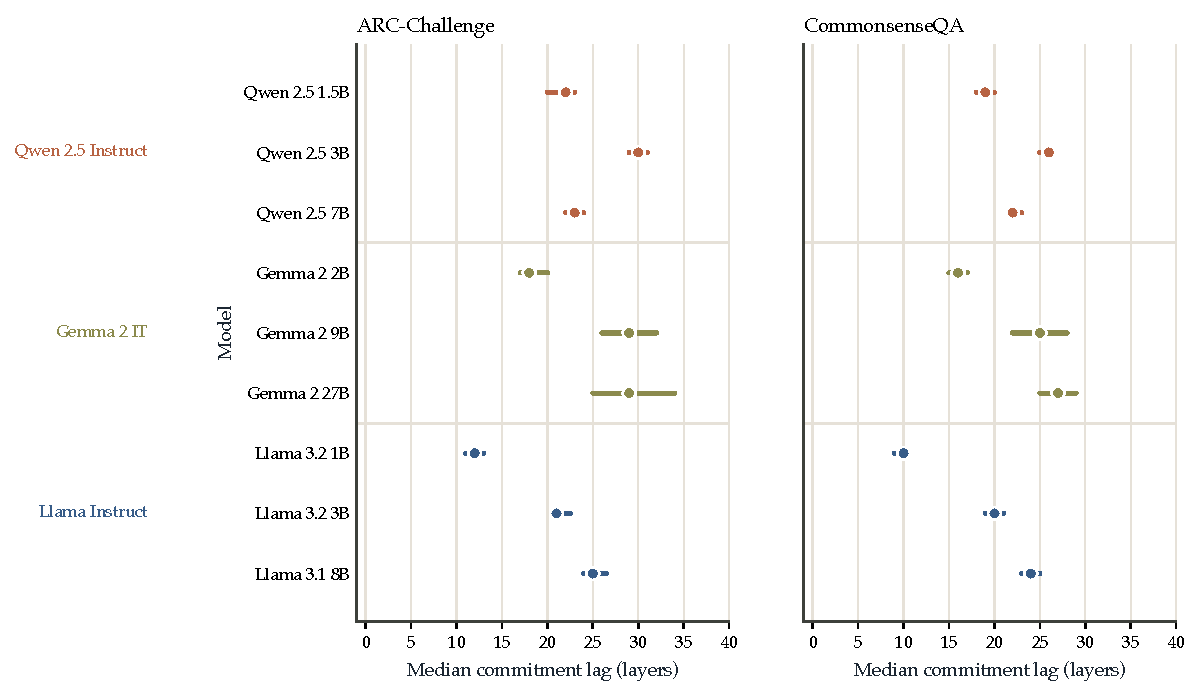
\includegraphics[width=\textwidth]{figure2_primary_forest_plot.pdf}
\caption{\textbf{Every evaluable ARC-Challenge and CommonsenseQA cell is positive under the preregistered primary rule.} Each point is the cell-level median commitment lag $\Delta_{\mathrm{margin}}$ in raw layer units for the primary analysis path, and each horizontal interval is a grouped-bootstrap 95\% confidence interval. Every reported model-dataset cell is positive.}
\label{fig:forest}
\end{figure*}

Figure~\ref{fig:forest} and Table~\ref{tab:primary-summary} translate the pooled picture
into the preregistered cell-level decision rule. All \ArcCsqaPositiveCells{} evaluable
ARC-Challenge and CommonsenseQA cells are positive, and there are no evaluated
negatives. So the main pattern is not just a pooled average. It survives at the level of
individual model-dataset cells.

\begin{table}[t]
\centering
\small
\begin{tabular}{@{}lccc@{}}
\toprule
Dataset & Positive & Evaluable & Insufficient \\
\midrule
ARC-Challenge & 9 & 9 & 0 \\
CommonsenseQA & 9 & 9 & 0 \\
All reported datasets & 18 & 18 & 0 \\
\bottomrule
\end{tabular}

\caption{\textbf{Primary-rule summary by dataset.} ARC-Challenge and CommonsenseQA are positive in every evaluable model-dataset cell.}
\label{tab:primary-summary}
\end{table}

The family-level summaries tell the same story. Qwen contributes six positive primary cells,
Gemma contributes six, and Llama contributes six. So the result is broad across the chosen
instruct-model panel, even though the exact lag size still varies with model depth and
dataset difficulty.

\FloatBarrier

\section{Controls and robustness}

The controls change only one thing: the exact string scored after ``\texttt{Final answer:}''.
Figure~\ref{fig:controls} shows why that matters. Under identity ordering, the primary
exact-option readout yields a \SemanticIdentityValidRate{} valid-rate for
$\Delta_{\mathrm{margin}}$. If we keep the prompt fixed but score the literal continuation
``\texttt{The answer is \{option\}}'' instead, that valid-rate falls to
\TemplatedIdentityValidRate{}. If we score only the answer letter, it rises to
\LetterIdentityValidRate{}.

The broad phenomenon does persist under both controls. On the fully paired identity subset,
the median lag is \SemanticPairedLagMedian{} layers for the exact-option readout,
\TemplatedPairedLagMedian{} layers for the templated control, and
\LetterPairedLagMedian{} layers for the letter-label control. The share of positive-lag cases
on that same paired subset is \SemanticPairedPositivePct{}, \TemplatedPairedPositivePct{},
and \LetterPairedPositivePct{}, respectively. So the main effect is not unique to one answer
format.

\begin{figure}[t]
\centering
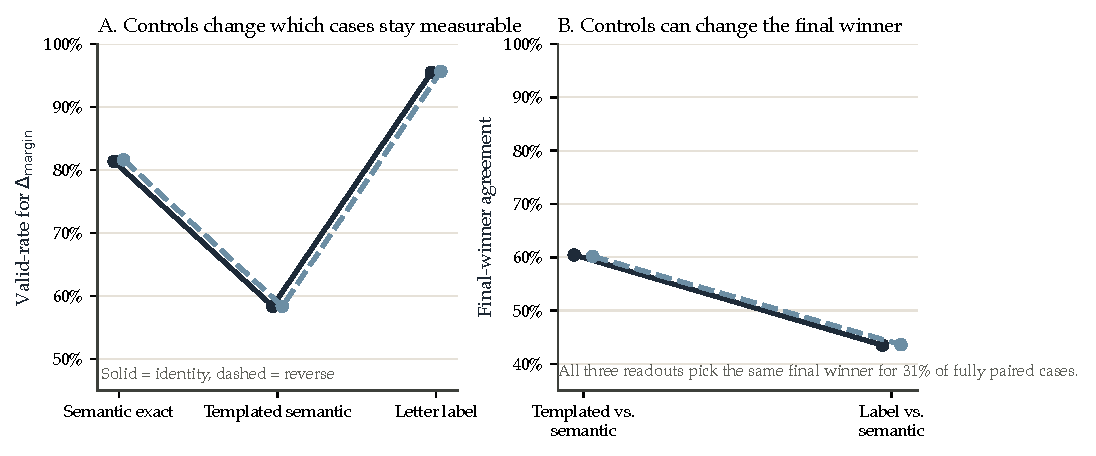
\includegraphics[width=\columnwidth]{figure3_control_readout_comparison.pdf}
\caption{\textbf{The broad lag survives the controls, but the controls still change the measurement.} Panel A shows how often $\Delta_{\mathrm{margin}}$ is defined for each readout. Panel B shows how often the two control readouts pick the same final winner as the semantic-exact primary readout on fully paired cases. Identity and reverse order behave similarly. The answer-format controls do not, which is why they are useful robustness checks but not replacements for the main semantic path.}
\label{fig:controls}
\end{figure}

The readouts also disagree on which answer the model prefers at the end. In fully paired
identity cases, the templated control agrees with the exact-option path on only
\TemplatedAgreementIdentity{} of cases, the letter-label control agrees on only
\LetterAgreementIdentity{}, and all three readouts agree on just \AllSameReadoutRate{} of
cases. This is exactly why we kept the controls. They tell us that the early-candidate /
late-commitment pattern is fairly robust, while also showing that different answer formats
can change the evaluable set and can even change the final winner. That makes the controls
scientifically useful, but it also means they are not interchangeable with the primary
exact-option analysis.

The answer-order control tells a different story. In Figure~\ref{fig:controls}, the identity
and reverse traces are nearly on top of each other. That is reassuring because it suggests
the main effect is not coming from one arbitrary option order. The report-only robustness
summaries also line up with the primary rule. The secondary criterion yields the same
positive pattern as the primary rule (\OverallSecondaryPositiveCells{} positive,
\OverallSecondaryInsufficientCells{} insufficient), and the gold-answer sensitivity analysis is
positive on all \GoldArcCsqaPositiveCells{} evaluable ARC-Challenge and CommonsenseQA
cells.

Finally, the QC path is designed to surface problems, not hide them. The released audit bundle logs \TokenCollisionCount{} tokenization collisions and \DuplicateOptionCount{} duplicate-option examples instead of silently dropping them, while the merged run itself still has zero failure rows and zero unpaired rows. The point is not to make the result look tidy. The point is to show that the result still holds when we keep the pipeline honest about edge cases.

\FloatBarrier

\section{Interpretation and limits}

Figure~\ref{fig:exemplars} shows what the aggregate result looks like in individual cases. Each panel plots the winner-minus-runner contrast for one semantic-exact identity example. The details differ by family and prompt, but the same broad pattern appears again and again: the eventual answer becomes plausible early, while stable commitment arrives much later and can be preceded by hesitation or reversals.

\begin{figure*}[t]
\centering
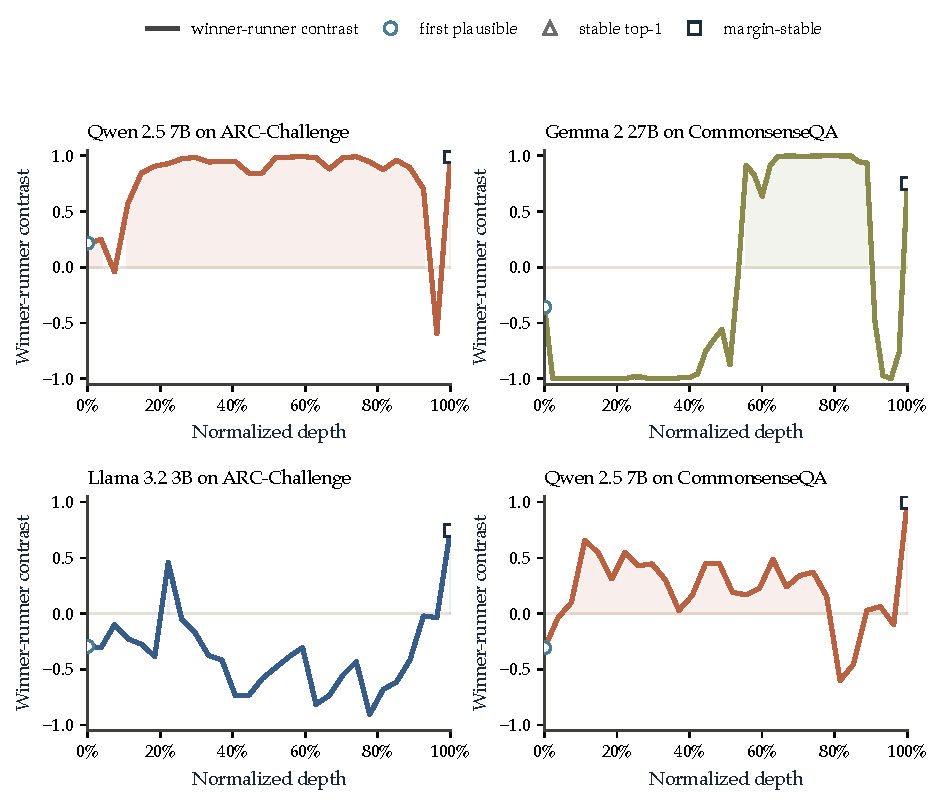
\includegraphics[width=\textwidth]{figure4_prompt_level_exemplars.pdf}
\caption{\textbf{Prompt-level trajectories show the same pattern as the pooled figures.} Each panel plots the winner-minus-runner contrast across normalized depth for one semantic-exact identity example. The circular marker shows when the eventual answer first enters the plausible set, the triangular marker shows when it becomes stable top-1, and the square marker shows when it becomes margin-stably committed. The exact shapes vary, but the same left-to-right separation between plausibility and commitment appears at the single-case level.}
\label{fig:exemplars}
\end{figure*}

These measurements still need to be interpreted carefully. We are not claiming that the model literally stores a human-like list of hypotheses, and we are not claiming that these curves identify a full causal circuit. Our claim is narrower. Under this prompting and scoring setup, the eventual answer often enters the plausible-answer set before it becomes stably isolated from the runner-up.

The empirical scope is also narrow in two practical ways. First, the paper uses a
\PaperPromptCount{}-question slice rather than the full benchmark splits. Second, the panel
contains only instruction-tuned open-weight models, so the claim should not be generalized
to base models or closed systems.

Those limits matter, but they do not erase the signal. The early-plausibility/late-commitment pattern appears in the pooled depth curves, in every evaluable ARC-Challenge and CommonsenseQA cell, and in the prompt-level trajectories. The controls matter here too. They show that small changes in answer format can change coverage and final winners, which is exactly why the paper keeps exact option-text scoring as the main path.

\FloatBarrier

\section{Conclusion}

The paper's claim is simple and deliberately scoped. In the setting we study,
instruction-tuned models often know which answers are still possible before they have fully
settled on the one they will finally say. We show that pattern by ending each prompt with
``\texttt{Final answer:}'' and tracking how the scores of exact answer continuations change
across model depth.

The evidence is consistent across levels of analysis. The flagship pooled curves show a large gap between plausibility and commitment. Every evaluable ARC-Challenge and CommonsenseQA model-dataset cell is positive under the preregistered primary rule. The prompt-level examples show the same separation in concrete trajectories. The answer-format controls matter because they show that this result is not automatic: changing the continuation string can change both coverage and winners.

The result does not yet explain why the gap appears, and it should not be overgeneralized beyond this panel and benchmark slice. But it does support a useful empirical distinction for future work. The moment when a model finally says an answer can come much later than the moment when that answer first becomes one of the answers the model already treats as plausible.


\bibliographystyle{colm2026_conference}
\bibliography{references}

\onecolumn
\appendix
\section{Supplementary material}

\subsection{Reproducibility statement}

This manuscript is generated from a single merged run, \texttt{\MergedRunId}, with
run-scoped manifests, QC summaries, and figure/table provenance checked into the paper
workspace. The reported analysis uses the ARC-Challenge and CommonsenseQA portion of
that run. All numeric claims in the paper are generated from those artifacts rather than
entered by hand.

\subsection*{Ethics statement}

This study analyzes public benchmark questions using open-weight language models and does
not involve human subjects, personal data, or deployment to end users. The main risk is
analytical overclaiming: layerwise statistics can be mistaken for a complete mechanistic
explanation when they are only an operational measurement. We mitigate that risk by
keeping the claim narrow, preregistering the primary rule, preserving anomaly logs, and
distinguishing the primary exact-option analysis from the control readouts.

\subsection*{AI-use disclosure}

AI-use disclosure. The authors used AI-assisted tools during the project lifecycle: ChatGPT for brainstorming and experimental design iteration, Codex for implementation assistance, and Claude Opus for drafting and formatting portions of the manuscript and LaTeX source. All scientific decisions, experiments, analyses, code review, result verification, and final manuscript editing were performed and approved by the human authors, who take full responsibility for the paper’s contents.

\subsection{Model registry}

\begin{center}
\small
\begin{tabularx}{\linewidth}{@{}lllXX@{}}
\toprule
Family & Model & Size & Repository & Revision prefix \\
\midrule
Qwen 2.5 Instruct & Qwen 2.5 1.5B & 1.5b & Qwen2.5-1.5B-Instruct & \texttt{989aa7980e4c} \\
Qwen 2.5 Instruct & Qwen 2.5 3B & 3b & Qwen2.5-3B-Instruct & \texttt{aa8e72537993} \\
Qwen 2.5 Instruct & Qwen 2.5 7B & 7b & Qwen2.5-7B-Instruct & \texttt{a09a35458c70} \\
Gemma 2 IT & Gemma 2 2B & 2b & gemma-2-2b-it & \texttt{299a8560bedf} \\
Gemma 2 IT & Gemma 2 9B & 9b & gemma-2-9b-it & \texttt{11c9b309abf7} \\
Gemma 2 IT & Gemma 2 27B & 27b & gemma-2-27b-it & \texttt{aaf20e6b9f4c} \\
Llama Instruct & Llama 3.2 1B & 1b & Llama-3.2-1B-Instruct & \texttt{9213176726f5} \\
Llama Instruct & Llama 3.2 3B & 3b & Llama-3.2-3B-Instruct & \texttt{0cb88a4f764b} \\
Llama Instruct & Llama 3.1 8B & 8b & Meta-Llama-3.1-8B-Instruct & \texttt{0e9e39f249a1} \\
\bottomrule
\end{tabularx}

\captionof{table}{\textbf{Model registry used in the paper.} Short repository names and 12-character revision prefixes are shown for readability; the full pinned revision hashes are preserved in the released provenance manifest.}
\label{tab:model-registry}
\end{center}

\subsection{Full primary positivity table}

\begin{center}
\scriptsize
\begin{tabularx}{\textwidth}{@{}llcccc@{}}
\toprule
Dataset & Model & Valid / total & Median lag & 95\% CI & Primary decision \\
\midrule
ARC-Challenge & Qwen 2.5 1.5B & 109/195 & 22 & [20, 23] & positive \\
ARC-Challenge & Qwen 2.5 3B & 143/195 & 30 & [29, 31] & positive \\
ARC-Challenge & Qwen 2.5 7B & 163/195 & 23 & [22, 24] & positive \\
ARC-Challenge & Gemma 2 2B & 117/195 & 18 & [17, 20] & positive \\
ARC-Challenge & Gemma 2 9B & 132/195 & 29 & [26, 32] & positive \\
ARC-Challenge & Gemma 2 27B & 135/195 & 29 & [25, 34] & positive \\
ARC-Challenge & Llama 3.2 1B & 79/195 & 12 & [11, 13] & positive \\
ARC-Challenge & Llama 3.2 3B & 104/195 & 21 & [20, 22] & positive \\
ARC-Challenge & Llama 3.1 8B & 112/195 & 25 & [24, 26] & positive \\
CommonsenseQA & Qwen 2.5 1.5B & 677/794 & 19 & [18, 20] & positive \\
CommonsenseQA & Qwen 2.5 3B & 706/794 & 26 & [25, 26] & positive \\
CommonsenseQA & Qwen 2.5 7B & 718/794 & 22 & [22, 23] & positive \\
CommonsenseQA & Gemma 2 2B & 693/794 & 16 & [15, 17] & positive \\
CommonsenseQA & Gemma 2 9B & 702/794 & 25 & [22, 28] & positive \\
CommonsenseQA & Gemma 2 27B & 706/794 & 27 & [25, 29] & positive \\
CommonsenseQA & Llama 3.2 1B & 625/794 & 10 & [9, 10] & positive \\
CommonsenseQA & Llama 3.2 3B & 672/794 & 20 & [19, 21] & positive \\
CommonsenseQA & Llama 3.1 8B & 649/794 & 24 & [23, 25] & positive \\
\bottomrule
\end{tabularx}

\captionof{table}{\textbf{Full cell-level primary-rule results.} The primary decision is evaluated separately for each model-dataset cell on the semantic-exact identity path.}
\label{tab:full-positivity}
\end{center}

\subsection{Selection and QC details}

\begin{center}
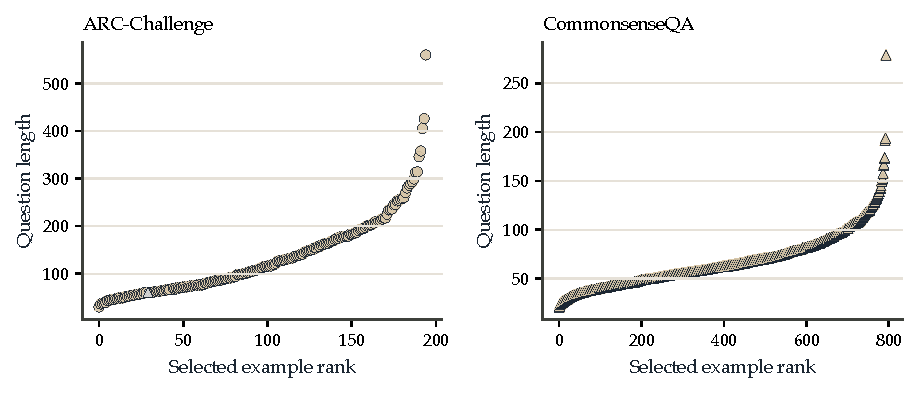
\includegraphics[width=\linewidth]{appendix_selection_profile.pdf}
\captionof{figure}{\textbf{The paper slice spans a wide range of selected prompt lengths.} The figure shows the selected-example question-length profile for each reported dataset together with the chosen option-count markers.}
\label{fig:selection}
\end{center}

\begin{center}
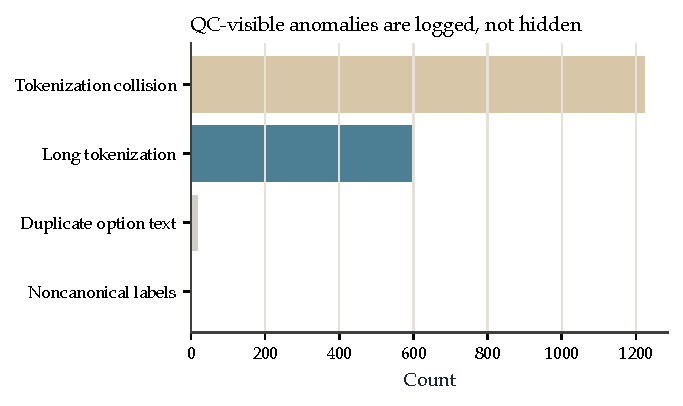
\includegraphics[width=\columnwidth]{appendix_qc_anomalies.pdf}
\captionof{figure}{\textbf{QC-visible anomalies are logged rather than hidden.} These counts come directly from the merged run's QC summary. They motivate caution, but they do not arise from silent exclusion or failed pairing.}
\label{fig:qc}
\end{center}

\begin{center}
\small
\begin{tabular}{@{}lc@{}}
\toprule
QC item & Count \\
\midrule
Prepared examples & 1000 \\
Token audits & 258876 \\
Tokenization collisions & 1224 \\
Suspiciously long option tokenizations & 594 \\
Duplicate option text & 17 \\
Noncanonical option labels & 2 \\
Unpaired rows & 0 \\
Failure rows & 0 \\
\bottomrule
\end{tabular}

\captionof{table}{\textbf{QC summary for the merged run.} The run completes with zero failure rows and zero unpaired rows while still surfacing tokenization and option-surface anomalies.}
\label{tab:qc-summary}
\end{center}

\begin{center}
\small
\begin{tabularx}{\linewidth}{@{}lXl@{}}
\toprule
Readout & Continuation surface & Normalization \\
\midrule
semantic\_exact & Exact option text after ``\texttt{Final answer:}'', e.g. ``\texttt{photosynthesis}'' & Mean log-probability \\
templated\_semantic & Literal continuation ``\texttt{The answer is \{option\_text\}}'' & Mean log-probability \\
letter\_label & Bare answer letter after ``\texttt{Final answer:}'', e.g. ``\texttt{A}'' & Mean log-probability \\
\bottomrule
\end{tabularx}

\captionof{table}{\textbf{Readout definitions used in the paper.} The controls intentionally differ in continuation surface while keeping the rest of the setup fixed.}
\label{tab:readout-defs}
\end{center}


\end{document}
